\documentclass[prb,twocolumn,showpacs,preprintnumbers,amsmath,amssymb, superscriptaddress]{revtex4-2}

%\usepackage[magyar]{babel}
%\usepackage[makeroom]{cancel}
\usepackage{amsmath}    % need for subequations
\usepackage{amssymb}
\usepackage{graphicx}   % need for figures
\usepackage{verbatim}   % useful for program listings
\usepackage{color}      % use if color is used in text
%\usepackage{subfigure}  % use for side-by-side figures
\usepackage{hyperref}   % use for hypertext links, including those to external documents and URLs
%\usepackage{blindtext}
\usepackage[normalem]{ulem}
%\usepackage{xpatch}
\usepackage{natbib}
\usepackage{fixmath}
\usepackage{enumitem}
\usepackage{dsfont}
\usepackage{subcaption}

\def \brc #1{\left\lbrace #1 \right\rbrace}
\def \loc {\mathrm{loc}}


\hypersetup{colorlinks,linkcolor=blue,urlcolor=blue,citecolor=blue}
\newcommand{\uv}[1]{\ensuremath{\mathbf{\hat{#1}}}} % for unit vector
\newcommand{\gv}[1]{\ensuremath{\mbox{\boldmath$ #1 $}}} % 
\newcommand{\rem}[1]{  {\color{red} #1}  }
%\newcommand{\g}[1]{{\bf #1 }} %
\newcommand{\beq}{\begin{equation}}
\newcommand{\eeq}{\end{equation}}
\newcommand{\bea}{\begin{eqnarray}}
\newcommand{\eea}{\end{eqnarray}}
\newcommand{\blabel}{\,b}
\newcommand{\alabel}{\,a}
\newcommand{\Lspace}{{\mathit{\mathbb{L}}}}

\newcommand{\bbGamma}{{\mathpalette\makebbGamma\relax}}
\newcommand{\makebbGamma}[2]{%
  \raisebox{\depth}{\scalebox{1}[-1]{$\mathsurround=0pt#1\mathbb{L}$}}%
}

\newcommand{\e}{\text e}
\newcommand{\zp}{\mathbb Z^+}
\newcommand{\z}{\mathbb Z}
\newcommand{\hint}{H_{\text{int}}}
\newcommand{\re}{\text{Re }}
\newcommand{\hc}{\text{h.c.}}
\newcommand{\cc}{\text{c.c.}}
\newcommand{\w}{\omega}
\newcommand{\be}{\begin{equation}}
\newcommand{\ee}{\end{equation}}
\newcommand{\Nedge}{N_{\rm edge}}



\definecolor{darkgreen}{rgb}{0,0.5,0}
\definecolor{orange}{rgb}{1,0.5,0}
\definecolor{grey}{rgb}{.6,.6,.6}
\newcommand{\rc}[1]{\textcolor{red}{#1}}
%\bibliographystyle{apsrev4-1}
%\newcommand{\jav}[1]{#1}
\newcommand{\scrap}[1]{{\color{orange}{\sout{#1}}}}
\newcommand{\cpm}[1]{{\color{blue}{#1}}}

\newcommand{\dr}{\text d^3r}
\newcommand{\dfi}{\text d\varphi}
\newcommand{\dd}{\text d}
\newcommand{\tr}{\tilde r}
\newcommand{\tn}{\tilde n}
\newcommand{\tz}{\tilde z}
\newcommand{\tc}{\tilde c}
\newcommand{\tS}{\tilde S}


\newcommand{\heff}{H_{\text{eff}}}
\newcommand{\hkin}{H_{\text{kin}}}

\newcommand{\pp}{P^{++}+P^{--}}
\newcommand{\ps}{P^{\text(S)}}
\newcommand{\pa}{P^{\text(A)}}
\newcommand{\psn}{P_{S=0}}
\newcommand{\pse}{P_{S=1}}
\newcommand{\eppn}{E^{+}_{0}}
\newcommand{\eppe}{E^{+}_{1}}
\newcommand{\ese}{E^{\text{(S)}}_{1}}
\newcommand{\esn}{E^{\text{(S)}}_{0}}
\newcommand{\eae}{E^{\text{(A)}}_{1}}
\newcommand{\ean}{E^{\text{(A)}}_{0}}
\newcommand{\kent}{k\in\text{NT}}
\newcommand{\meV}{\,{\rm meV}}
\newcommand{\ie}{{\it i.e. }}
\newcommand{\bra}[1]{\langle #1|}
\newcommand{\ket}[1]{|#1\rangle}
\newcommand{\average}[1]{\langle #1\rangle}

%\newcommand{\scrap}[1]{{\color{red}{\sout{#1}}}}


\newcommand{\bK}{\mathbf K}
\newcommand{\bS}{\mathbf S}
\newcommand{\bk}{\mathbf k}
\newcommand{\bq}{\mathbf q}
\newcommand{\ba}{\mathbf a}
\newcommand{\bC}{\mathbf C}
\newcommand{\bH}{\mathbf H}


\newcommand{\bx}{\mathbf x}
\newcommand{\br}{\mathbf r}
\newcommand{\brp}{{\mathbf r}'}
\newcommand{\bxp}{{\mathbf x}'}


\newcommand{\g}{{\gamma}}
\newcommand{\ds}{\displaystyle}
\newcommand{\1}{{1\hspace*{-0.5ex} \textrm{l} \hspace*{0.5ex}}}

\newcommand{\cL}{{\cal L }}
\newcommand{\fL}{\mathfrak{ L }}
\newcommand{\cH}{{\cal H }}
\newcommand{\fH}{\mathfrak{H }}

\newcommand{\cQ}{{\cal Q}}
\newcommand{\cG}{{\cal G}}
\newcommand{\cg}{{\cal g}}
\newcommand{\cS}{{\cal S}}
\newcommand{\cJ}{{\cal J}}
\newcommand{\cN}{{\cal N}}
\newcommand{\chU}{\hat{\cal U}}
\newcommand{\hU}{{\hat U}}

\newcommand{\ketL}[1]{|#1 )}
\newcommand{\braL}[1]{( #1|}
\newcommand{\averageL}[1]{( #1 )}
\newcommand{\tsigma}{{\tilde \sigma}}

\def\doubleunderline#1{\underline{\underline{#1}}}

\newcommand{\mk}[1]{{\color{blue} #1}}


\newcommand{\tp}[1]{{\color{darkgreen} #1}}

\begin{document}
\title{Theoretical modeling of the collective tunneling of a Wigner necklace}
\author{Dominik  Szombathy}
\affiliation{Department of Theoretical Physics,  Institute of Physics, Budapest University of Technology and Economics,  Budafoki \'ut 8., H-1111 Budapest, Hungary}
\affiliation{MTA-BME Quantum Dynamics and Correlations Research Group, 
Institute of Physics, Budapest University of Technology and Economics,  Budafoki \'ut 8., H-1111 Budapest, Hungary}
\author{Mikl\'os Antal Werner}
\affiliation{Department of Theoretical Physics,  Institute of Physics, Budapest University of Technology and Economics,  Budafoki \'ut 8., H-1111 Budapest, Hungary}
\affiliation{MTA-BME Quantum Dynamics and Correlations Research Group, 
Institute of Physics, Budapest University of Technology and Economics,  Budafoki \'ut 8., H-1111 Budapest, Hungary}
\author{C\u at\u alin Pa\c scu Moca}
\affiliation{Department of Theoretical Physics, Institute of Physics, Budapest University of Technology and Economics, Budafoki \'ut 8., H-1111 Budapest, Hungary}
\affiliation{Department of Physics, University of Oradea,  410087, Oradea, Romania}
\author{Gergely Zar\'and}
\affiliation{Department of Theoretical Physics,  Institute of Physics, Budapest University of Technology and Economics,  Budafoki \'ut 8., H-1111 Budapest, Hungary}
\affiliation{MTA-BME Quantum Dynamics and Correlations Research Group, 
Institute of Physics, Budapest University of Technology and Economics,  Budafoki \'ut 8., H-1111 Budapest, Hungary}
%\affiliation{ BME-MTA Exotic Quantum Phases Group, Institute of Physics, 
%Budapest University of Technology and Economics, H-1111 Budapest, Hungary}
\date{\today}
\begin{abstract}
To be written. 
\end{abstract}
\maketitle

\section{Introduction}
\begin{itemize}
\item Nanotube description
\item Experimental background
\item Wigner Crystal and $r_s$ values in this system
\end{itemize}

\begin{figure}[h!]
    \begin{center}
     \includegraphics[width=0.7\columnwidth]{Experimental_Setup.png}
     \vskip 10pt
     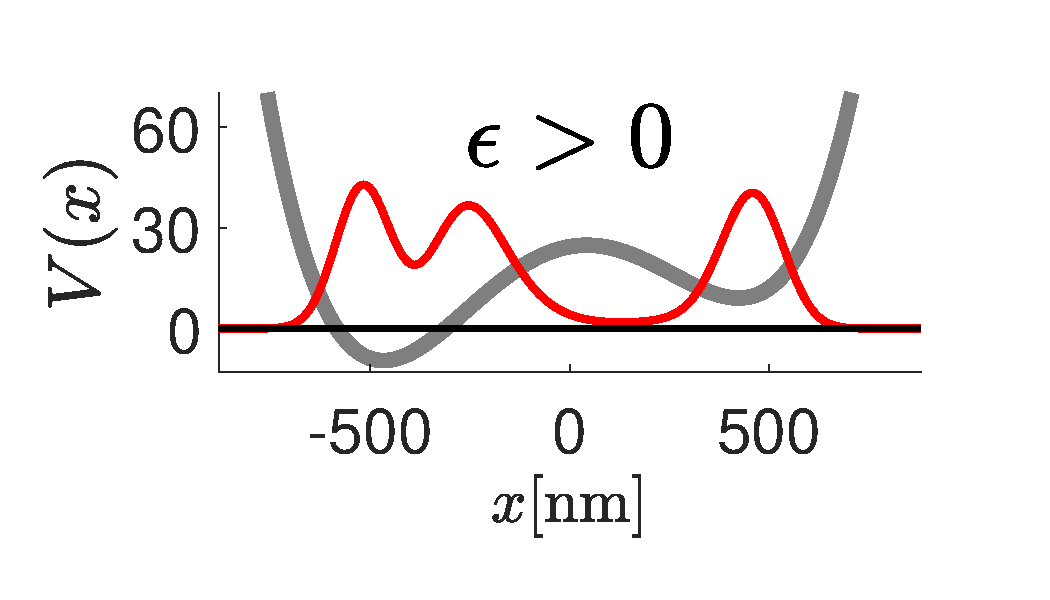
\includegraphics[width=0.49\columnwidth]{Fig_WaveFunction_Potential_NegEps_v1}
     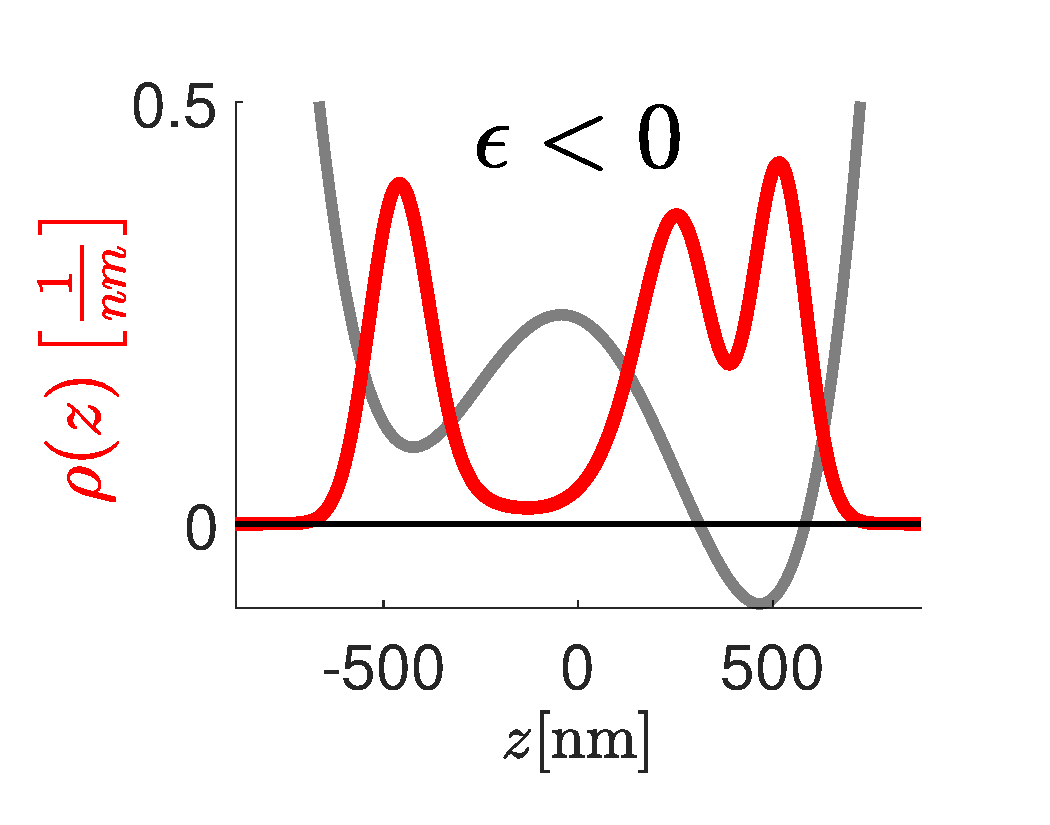
\includegraphics[width=0.49\columnwidth]{Fig_WaveFunction_Potential_PosEps}
    \end{center}
    \caption{Top: Sketch of  the experimental setup used to measure the
	 collective tunneling. The gates  
	 $V_{gi}$ are used to shape the double well potential. 
	 The lefthand side of the nanotube is used as a charge detector. 
	 Bottom: Ground state charge densities  (red) obtained via exact diagonlization  for a the double well potential (grey) with 3 electrons, in the case of finite detuning, $\epsilon = \pm 0.1 {\rm{ V/nm}}$, $\eta = 20$ dimensionless interaction parameter, see \eqref{dimless_interaction_param}. eq, plotted using the $l_d = 160 {\rm{ nm}}$ lengthscale.}
     \label{fig:experimental_setup}
\end{figure}
  
 \begin{figure}[h!]
    \begin{center}
    	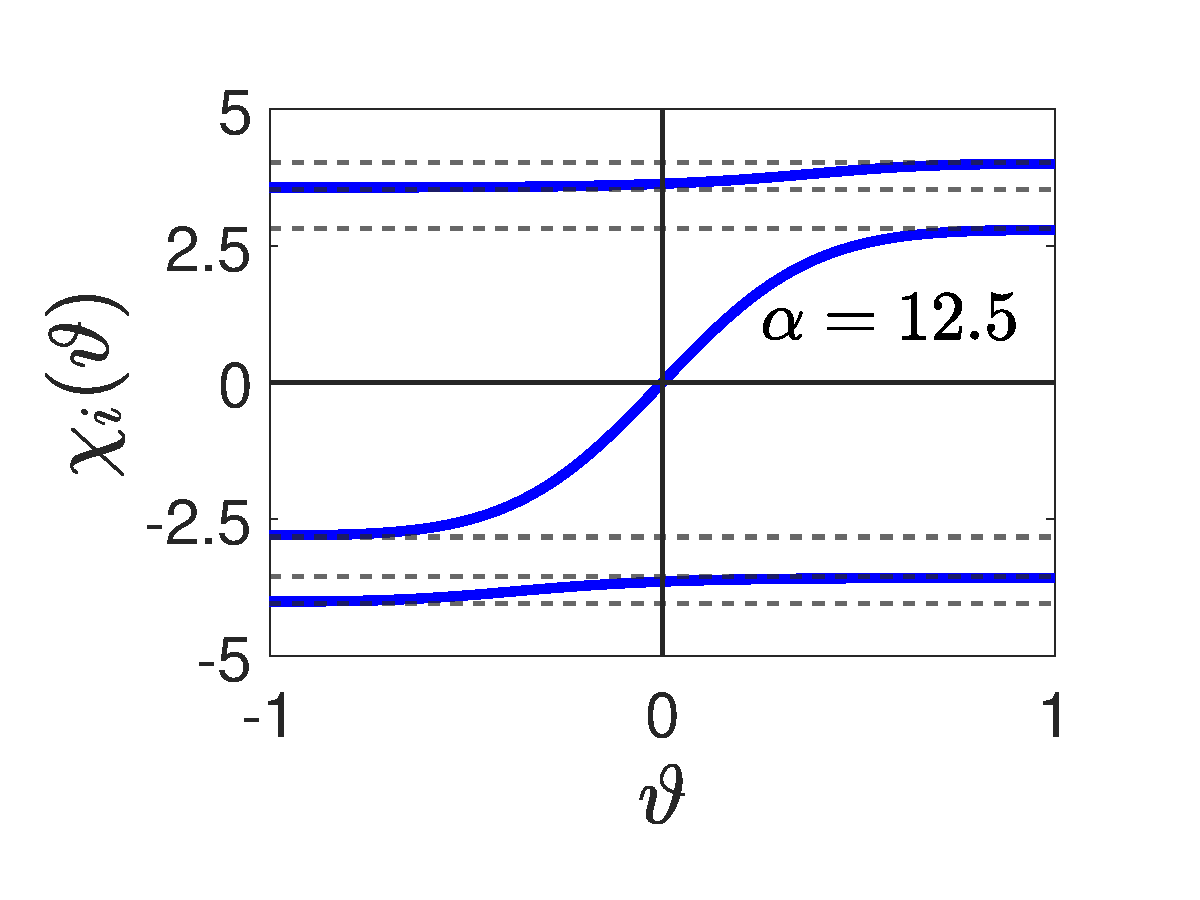
\includegraphics[width=0.8\columnwidth]{Fig_3Particle_Trajectory}
     	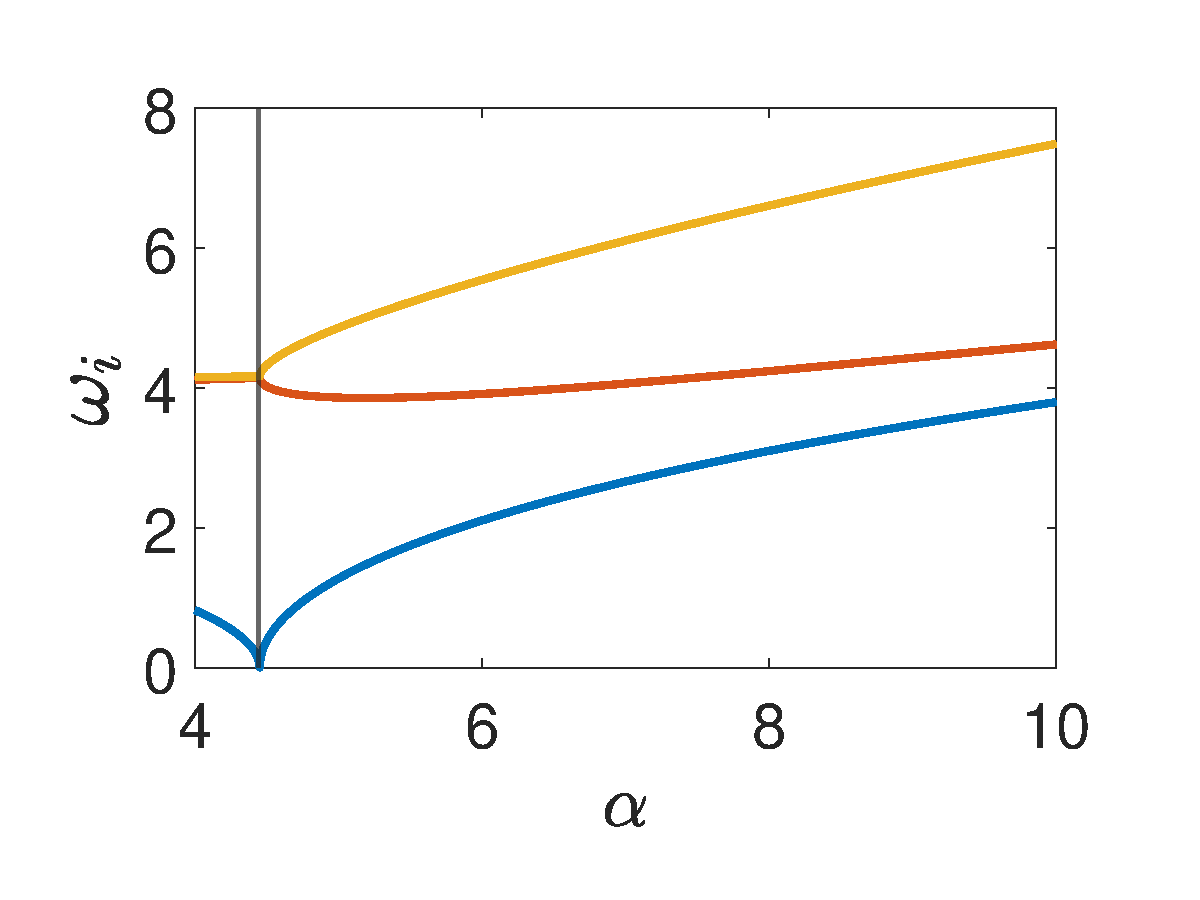
\includegraphics[width=0.8\columnwidth]{Fig_Freqs.pdf}

     \caption{Top: Three particle imaginary time trajectories (blue) in the dimensionless units for a specific confinement parameter $\alpha = 12.5$ and $\eta = 20$. Dashed lines show the classical equilibrium positions or instanton turning points for the 3 particles. Bottom: Eigenfrequencies as a function of $\alpha$, for three particles. The vertical line at $\alpha_{cr} \approx 4.45$ marks the beginning of the tunneling regime. For $\alpha > \alpha_{cr}$ two stable positions exist, and the particles move between these by collective tunneling.}
     \label{fig:experimental_setup}
    \end{center}
\end{figure}  

\begin{figure*}[h!]
    \begin{center}
    	\begin{tabular}{cc}
    		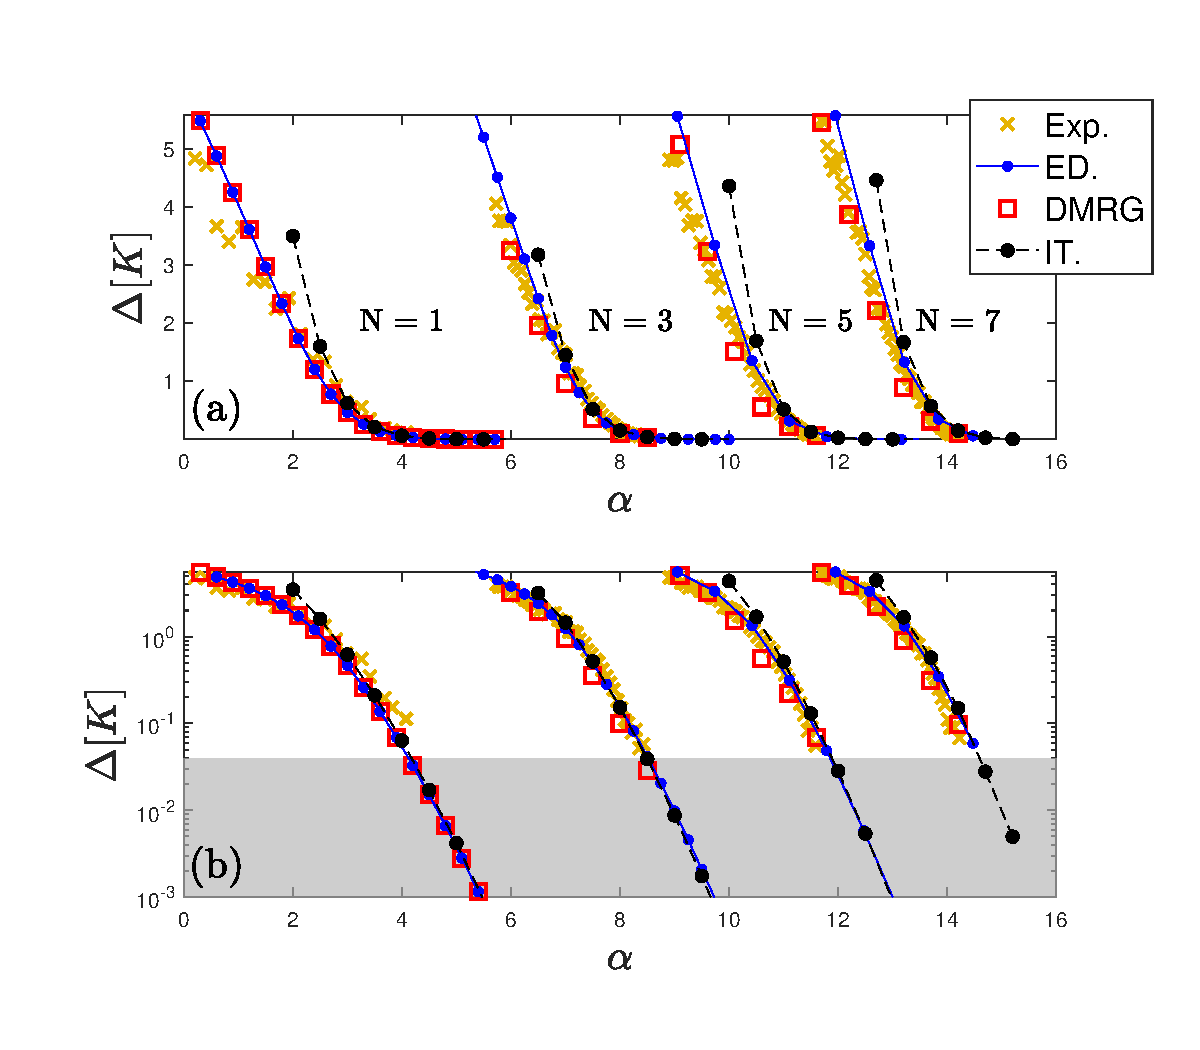
\includegraphics[width=1\columnwidth]{Fig_spectral_gap_exp_fitted_2}
     		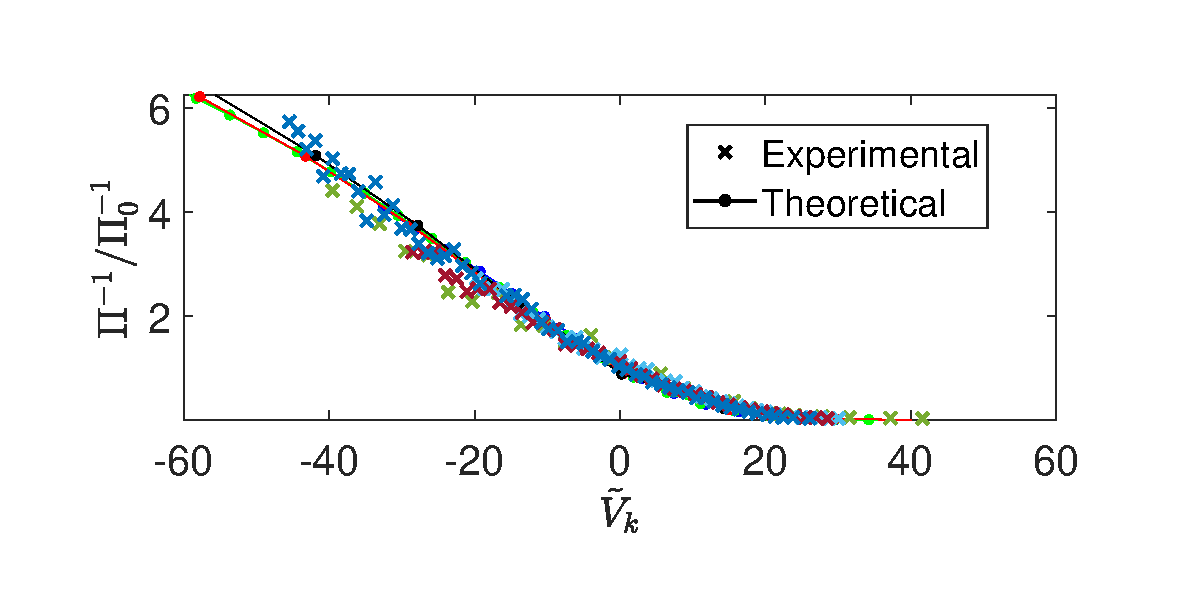
\includegraphics[width=1\columnwidth]{Fig_spectral_gap_exp_log_lin_shahal_scaling_log}
    	\end{tabular}
    	


		 	\caption{(a) and (b) Scaled experimental data for the measured polarization and numerical data for the tunnel splitting using various approaches as function the confinement parameter $\alpha$ that controls the hight of the barrier between the wells. Different curves correspond to different number of electrons in the system. (c) Perpendicular tunneling renormalization factor $R_0$ calculated from the instanton theory. (d) Demonstraition of the universal scaling between the experimental data and the exact diagonalization calculation. Gate voltage $V_k$ adjusts the potential barrier, and $\Pi_0^{-1}$ is a normalization factor obtained from the experimental curves critical $V_k$ value. (I kept it in it's original form from Shahal's ppt) }
     
     \label{fig:experimental_setup}
    \end{center}
\end{figure*}    
  	

\section{Numerical approaches}
\begin{itemize}
\item Effective Hami
\item alpha values; epsilon values
\item what we calculate, trajectories, tunnel splitting, polarization
\end{itemize}

\begin{equation}\label{dimfull_Hamiltonian}
H = \sum_{i = 1}^n \left[ -\frac{\hbar^2}{2m}\frac{\partial^2}{\partial z_i^2} + \frac{a}{2} z_i^2 + \frac{b}{4}z_i^4 + {c} z_i  \right] + \sum_{i<j}^n \frac{e^2}{4 \pi \varepsilon_0}\frac{1}{\left| z_i - z_j  \right|}
\end{equation}

\begin{equation}
\frac{z_i}{l_d} = \chi_i
\end{equation}

\begin{align}\label{dimless_Hamiltonian}
\frac{H}{E_0} &= \tilde{H} \\
 &= \sum_{i = 1}^n \left[ -\frac{1}{2}\frac{\partial^2}{\partial \chi_i^2} - \frac{\alpha}{2}\chi_i^2 + \frac{1}{4} \chi_i^4 + \epsilon \chi_i \right] + \eta \sum_{i < j}^n \frac{1}{\left| \chi_i - \chi_j  \right|}
\end{align}


\begin{equation}
l_d = \left( \frac{\hbar^2}{m^* \beta} \right)^{1/6} \approx 160 \,{\rm{ [nm]}}
\end{equation}
\begin{equation}
E_0 = \frac{\hbar^2}{m^* l_d^2} \approx 0.48 \,{\rm{ [meV]}}
\end{equation}

\begin{equation}\label{dimless_interaction_param}
\eta = \frac{l_d}{a_B} \approx 20
\end{equation}

\begin{align}
{\text{"Universal scaling"}}\\
v &= (V - \delta V_{n})/V_n \\
\tilde{\Delta} &= \Delta\, f_\Delta \\
\tilde{\alpha} &= (\alpha - \alpha_0^{(n)}) f_{\alpha, n} \\
{\text{Scaling to }} \alpha \\
\alpha(V) &= \delta\alpha_n + \frac{1}{V_0} \left(V - \delta V_n  \right)
\end{align}

\begin{table}[h!]
\begin{tabular}{|c|c|c|c|c|}
\hline
$n$ & $f_\alpha$   & $\delta V_n$ [mV] & $V_n$ [mV]  & $\alpha_0$ \\ \hline
1 & 14.8  & 109  & 1    & 2.2     \\ \hline
3 & 18.5  & 280  & 0.25 & 6.9     \\ \hline
5 & 21.28 & 560  & 0.15 & 10.4    \\ \hline
7 & 22.2  & 850  & 0.13 & 13.2    \\ \hline
\end{tabular}
\end{table}

\subsection{Instanton}

Path integral formalism gives great insight of quantum tunneling. The behaviour of the particle is described by the sum of all possible paths that it can take between two points in the potential. Each of these paths is weighted by their respective action.

\begin{figure}[h!]
		\begin{center}
			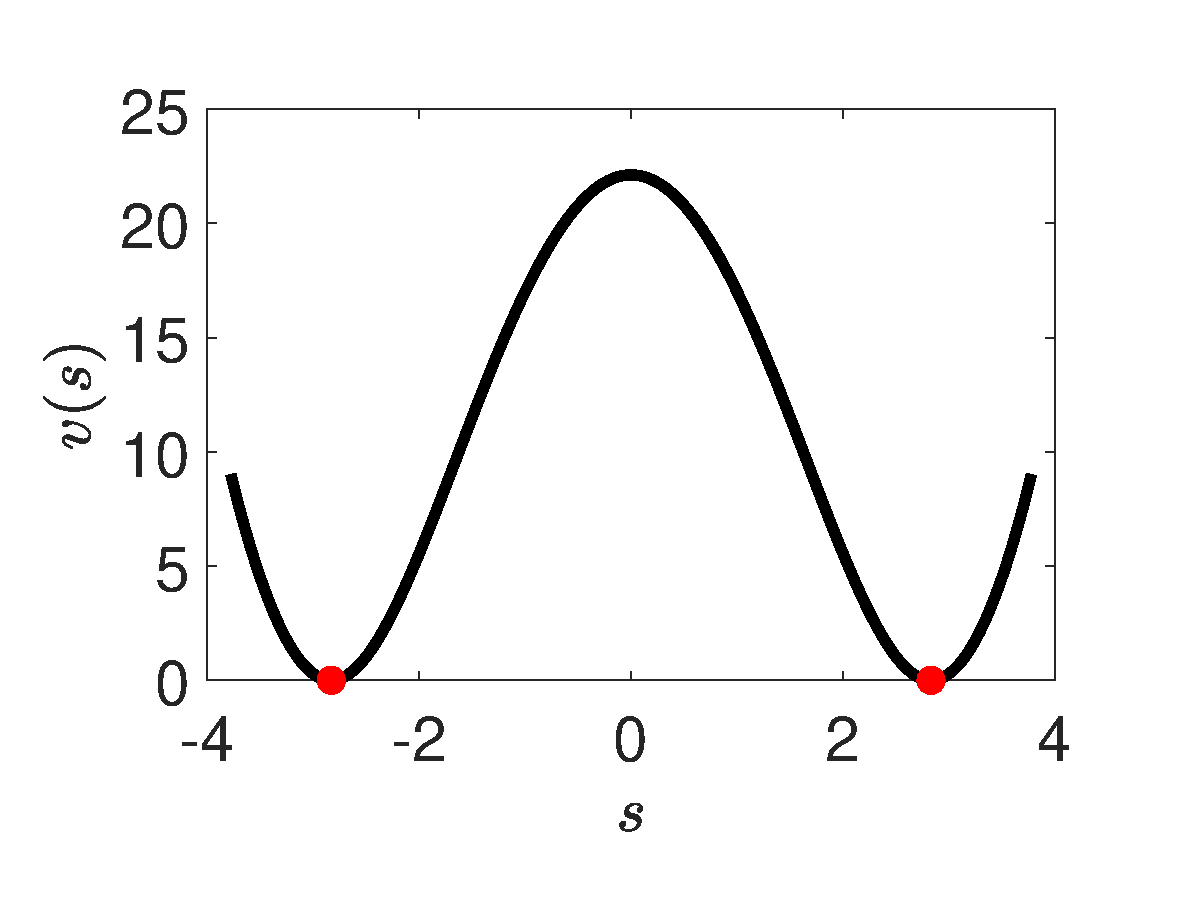
\includegraphics[width=0.9\columnwidth]{SupMatFig_EffectivePotential.pdf}
			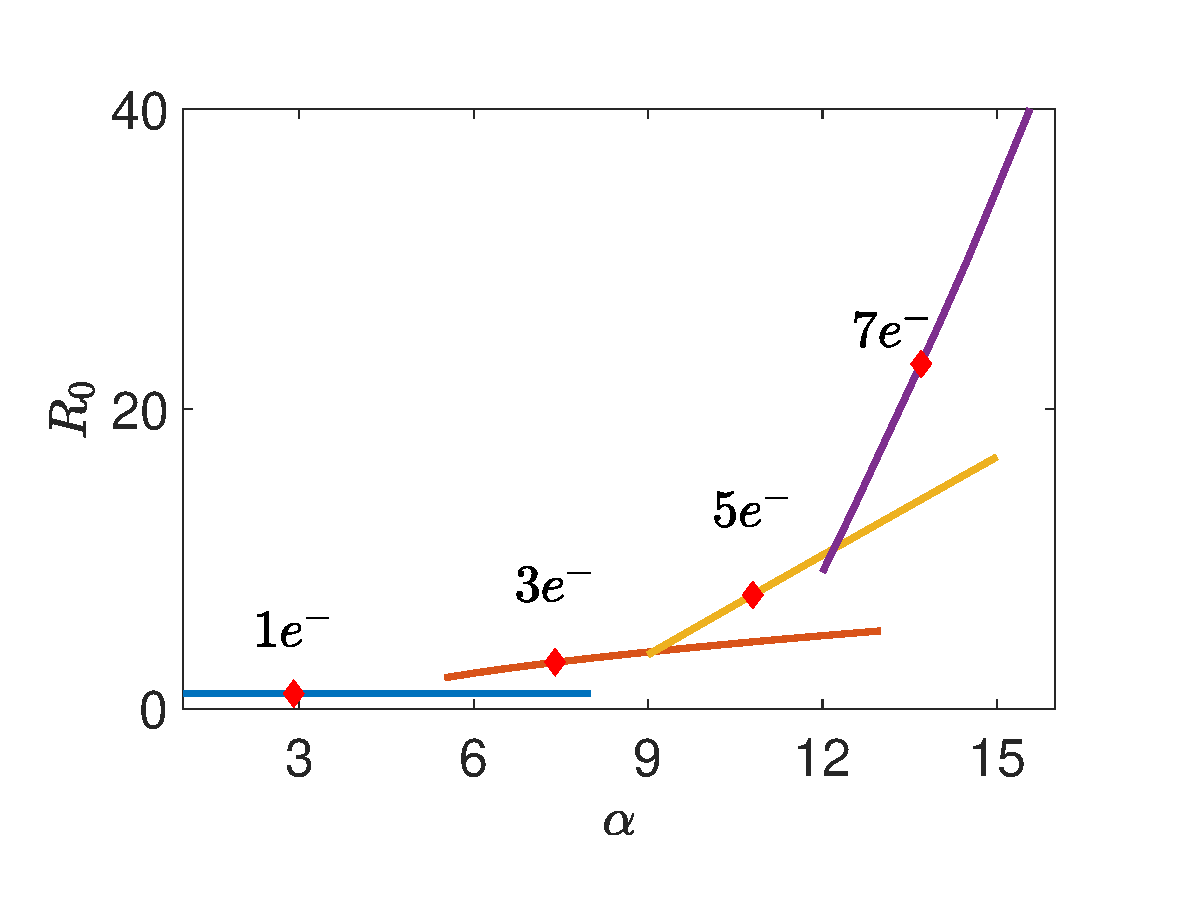
\includegraphics[width=0.9\columnwidth]{Fig_perpfactors.pdf}
			
			\label{fig:gap}
			\caption{Effective one-dimensional potential $v(s)$ for $N = 3$ particles, with $ds^2 = \sum_i d\chi_i^2$, for the arc length along the instanton trajectory for $\alpha = 10.5$ and $\eta = 20$.  }
		\end{center}
	\end{figure}

\begin{itemize}
\item summary of the calculation (details could go to appendix); Gergely's note: The calculation should be reproducable after reading this part. Include the numerical tricks here and for the ED as well.
\item Zero mode solution
\item Monte Carlo simulation details
\item Validity under a certain alpha
\item Perpendicualr factor
\end{itemize}

\begin{equation}
K(x,x^\prime,t) = \int\limits_{x^\prime (t_0)}^{x(t)} \mathcal{D}x \,\, e^{i\frac{1}{\hbar} \int {\rm{d}}t \mathcal{L}(x,\dot{x})}
\end{equation}

\begin{equation}
K(x,x^\prime,T) = e^{iS_{cl}} \int\limits_{r(0) = 0}^{r(T) = 0} \mathcal{D}\textbf{r} e^{\frac{1}{2} \int_0^T {\rm{d}} t \textbf{r}(t) \left[ m^\star \partial_\tau^2 + \partial^2 V(\textbf{x}_{cl}(t)) \right] \textbf{r}(t)}
\end{equation}


\begin{equation}
v_n(\{\chi_i\}_{i=1}^n) = \sum_{i=1}^n \left(-\frac{\alpha}{2} \chi_i^2 + \frac{1}{4} \chi_i^4   \right) + \eta \sum_{i < j}^n \frac{1}{|\chi_i - \chi_j |}
\end{equation}

\begin{equation}
S(\chi) = E_0 \int {\rm{d}}t \left\lbrace \frac{1}{2E_0^2} \left( \frac{{\rm{d}}\chi}{{\rm{d}}t} \right)^2 - v_n(\{\chi_i\}_{i=1}^n) \right\rbrace
\end{equation}

\begin{equation}
S_E = S_0 \sum_{i = 1}^n \int\limits_{-1 + \varepsilon}^{1 - \varepsilon} {\rm{d}}\vartheta \left\lbrace \frac{(1 - \vartheta^2)}{2\varrho} \left( \frac{{\rm{d}}\chi_i}{{\rm{d}}\vartheta} \right)^2  + \frac{\varrho}{1 - \vartheta^2} v_n(\{\chi_i\}_{i=1}^n) \right\rbrace
\end{equation}

\begin{equation}
t \rightarrow -i\tau
\end{equation}

\begin{equation}
iS \rightarrow -S_E
\end{equation}

\begin{equation}
\vartheta = \tanh\left( \frac{\tau E_0}{\hbar \varrho} \right)
\end{equation}

\begin{equation}
\Delta = R_0 \sqrt{\frac{4\omega_0}{\pi}} P\left[ \textbf{$\chi$}(\vartheta) \right] e^{-S_E}
\end{equation}

\begin{align}
B &= \sqrt{ \frac{2S_0}{\pi}} \left[ \frac{det^\prime \left(-\partial_\tau^2 + V^{\prime \prime}_0 (s_0 (\tau))   \right)}{det\left(-\partial_\tau^2 + \omega^2_N   \right)}  \right]^{-1/2}\\
&\times \left[  \frac{det^\prime \left(-\partial_\tau^2 {\bf{1}} + {\bf{\Omega}}^2 (\tau)   \right)}{det\left(-\partial_\tau^2 {\bf{1}}+ {\bf{\Omega}}^2_0   \right)}   \right]^{-1/2}
\end{align}

\begin{equation}
\Omega^2_{\alpha, \beta} (y) = \tau_\alpha {\bf{B}} \tau_\beta^T - 3 \tau^\prime_\alpha \tau_N \tau^\prime_\beta \tau_N
\end{equation}

\begin{equation}
{\bf{\dot{\Xi}}} = {\bf{\Omega}^2}(y) - {\bf{\Xi}}^2(y)
\end{equation}

\subsection{ED}
\begin{itemize}
\item general finite difference method description
\item restricted space method
\end{itemize}


Numerical solution of the Schrödinger equation is a powerfull tool in one-dimension or for effectively one-particle problems. In order to obtain the tunnel splitting, we have calciulated the energy difference between the ground state and first excited state for $N = [1, 3, 5, 7]$ particles using finite-difference methods. Efficent discretization of the state space, whihc is in our case is the dimensionless space $\chi_i$, determined by the calssical equilibrium positions of the fourth order potential. This is indeed important for the propernormalization conditions for the resulting wavefunctions, that is, we required that $\Psi_n$, which is the solution of $H_n \Psi_n = E_{i, n} \Psi_n$, decays exponentially at the edges of the numerical state space. In the Wigner crystal present the electrons becomes locaized and thus the describpiton of the i-th elcectron wavefunction does not extend over the whole state space, enableing us to restict the state space for certain electrons in the chain. With this restriction we were able to construct the $N$ particle Hamiltonian and calculate the necessary energy levels for the tunnel splitting.

\begin{equation}
\tilde{P} = \sum_{i=1}^n \int\limits_{-\infty}^{\infty} \Psi^\star_i (\chi) \chi \Psi_i(\chi)
\end{equation}

\begin{equation}
\rho(\chi) = \sum_{i=1}^n \Psi^\star_i (\chi) \Psi_i(\chi)
\end{equation}
\subsection{DMRG}
\begin{itemize}
\item Basis used
\item I guess technical description here is not that important, myabe in the SUpMat
\end{itemize}


\section{Results}
\subsection{Tunnel Splitting}

\subsection{Charge distribution and polarization}
\begin{figure}[h!]
    \begin{center}
     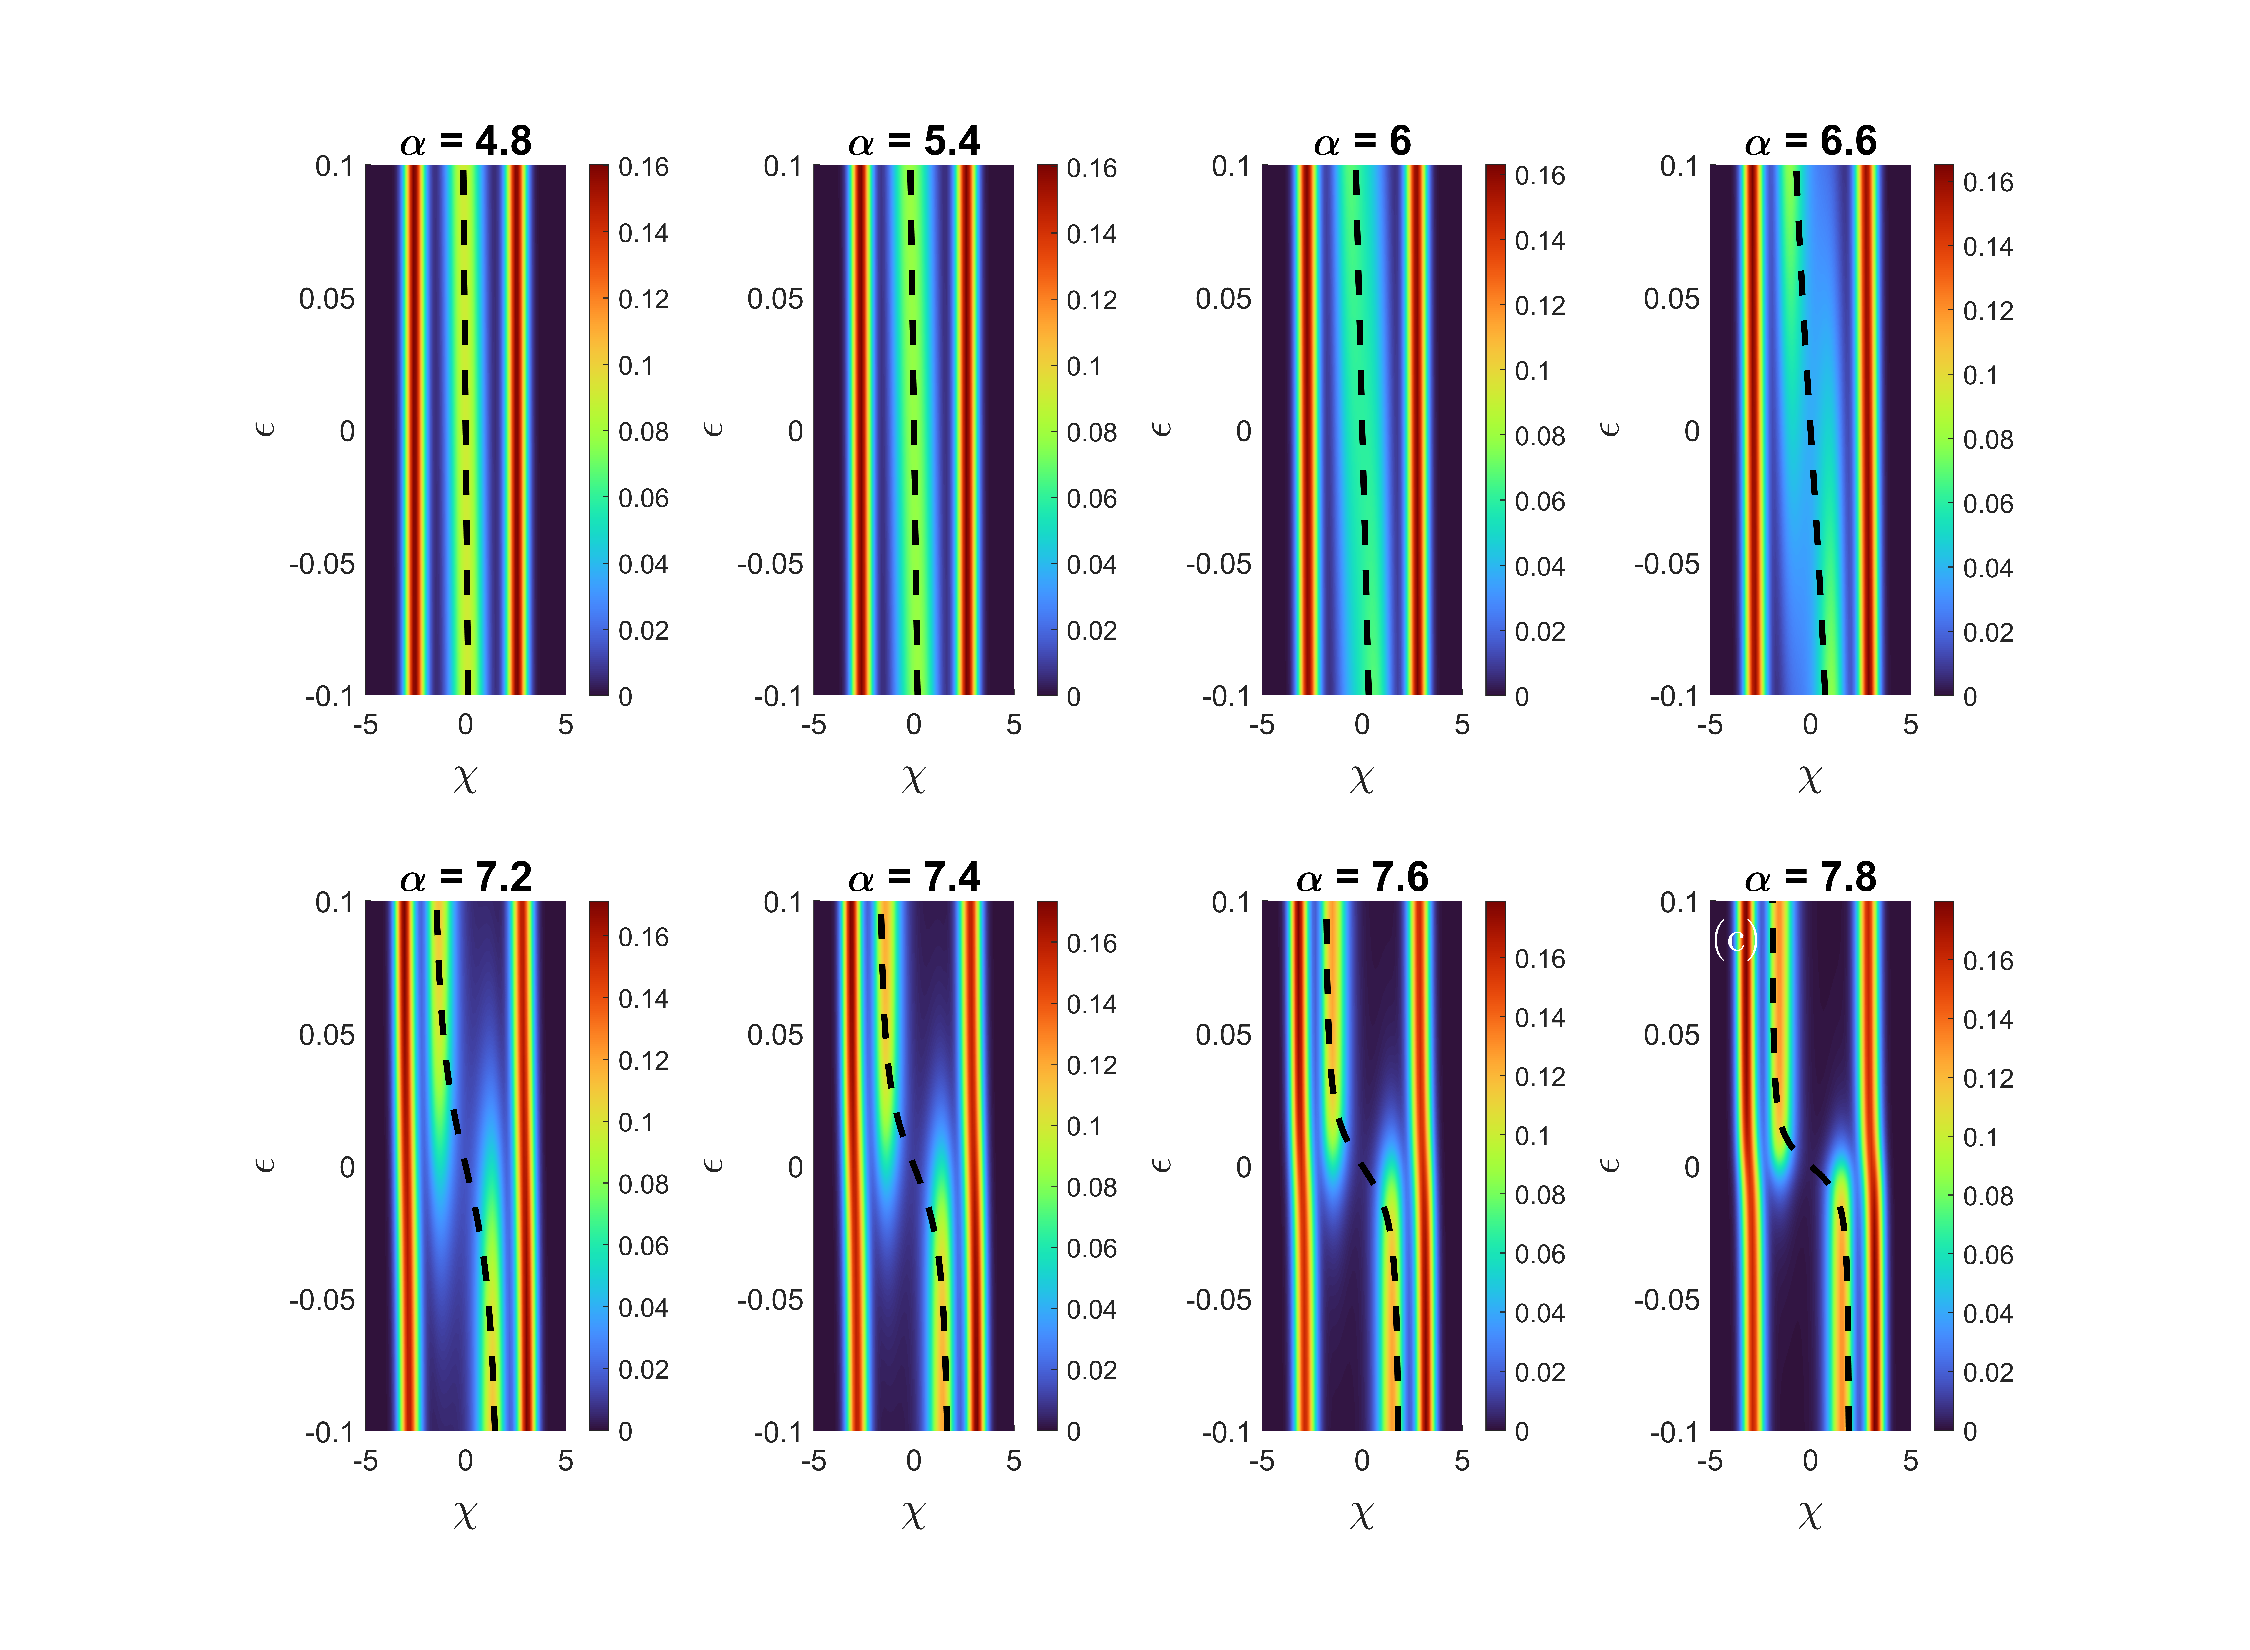
\includegraphics[width=2\columnwidth]{SupMatFig_DensitySeries}
     \label{fig:experimental_setup}
     \caption{Polarization series for $N = 3$ particles. The classical critical point is at $\alpha_{cl}^{N=3} \approx 4.45$, but tunneling occurs above $\alpha = 6$.}
     
    \end{center}
     \end{figure}

\begin{figure}[h!]
	\begin{center}
		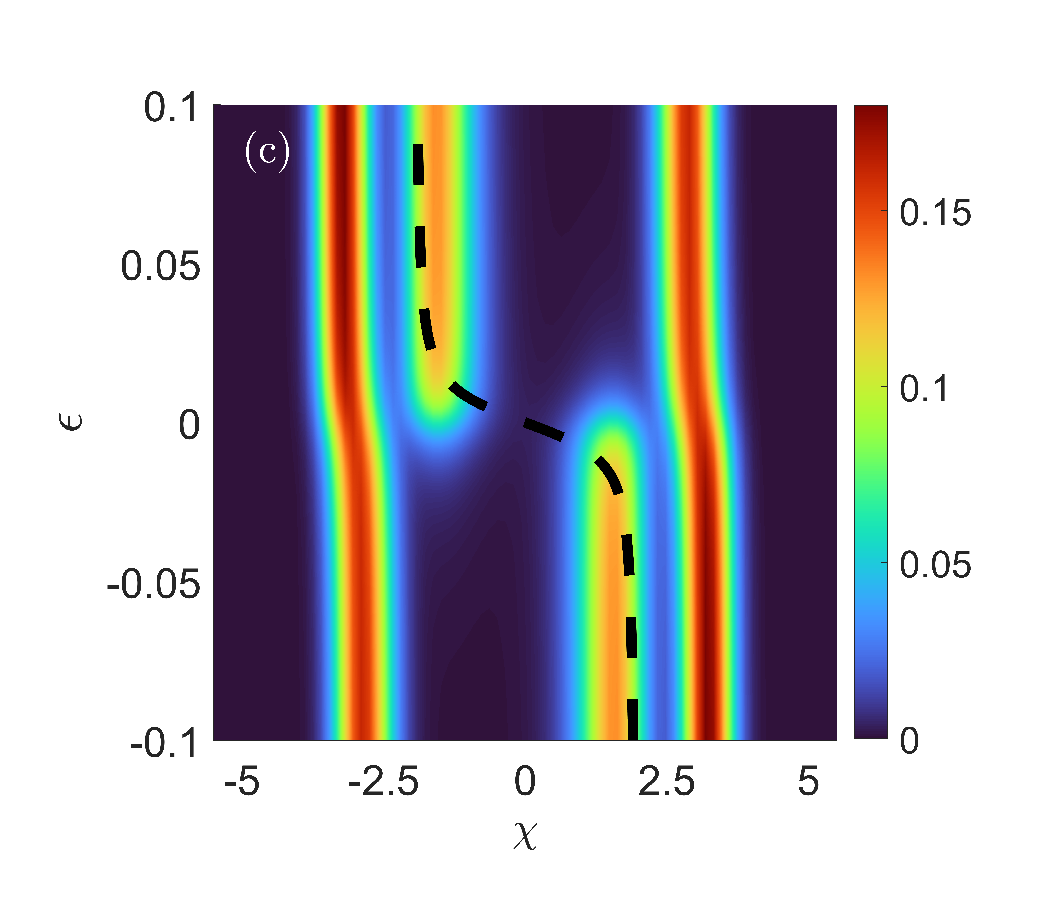
\includegraphics[width=1\columnwidth]{Fig_Polarization_2D}
		
		\caption{Top: Charge density as a function of the dimensionless electric field $\epsilon$ at $\alpha = 7.8$ and $\eta = 20$. The dashed line denotes the polarization in the system.}
	\end{center}
\end{figure}


\begin{figure}
	\begin{center}
	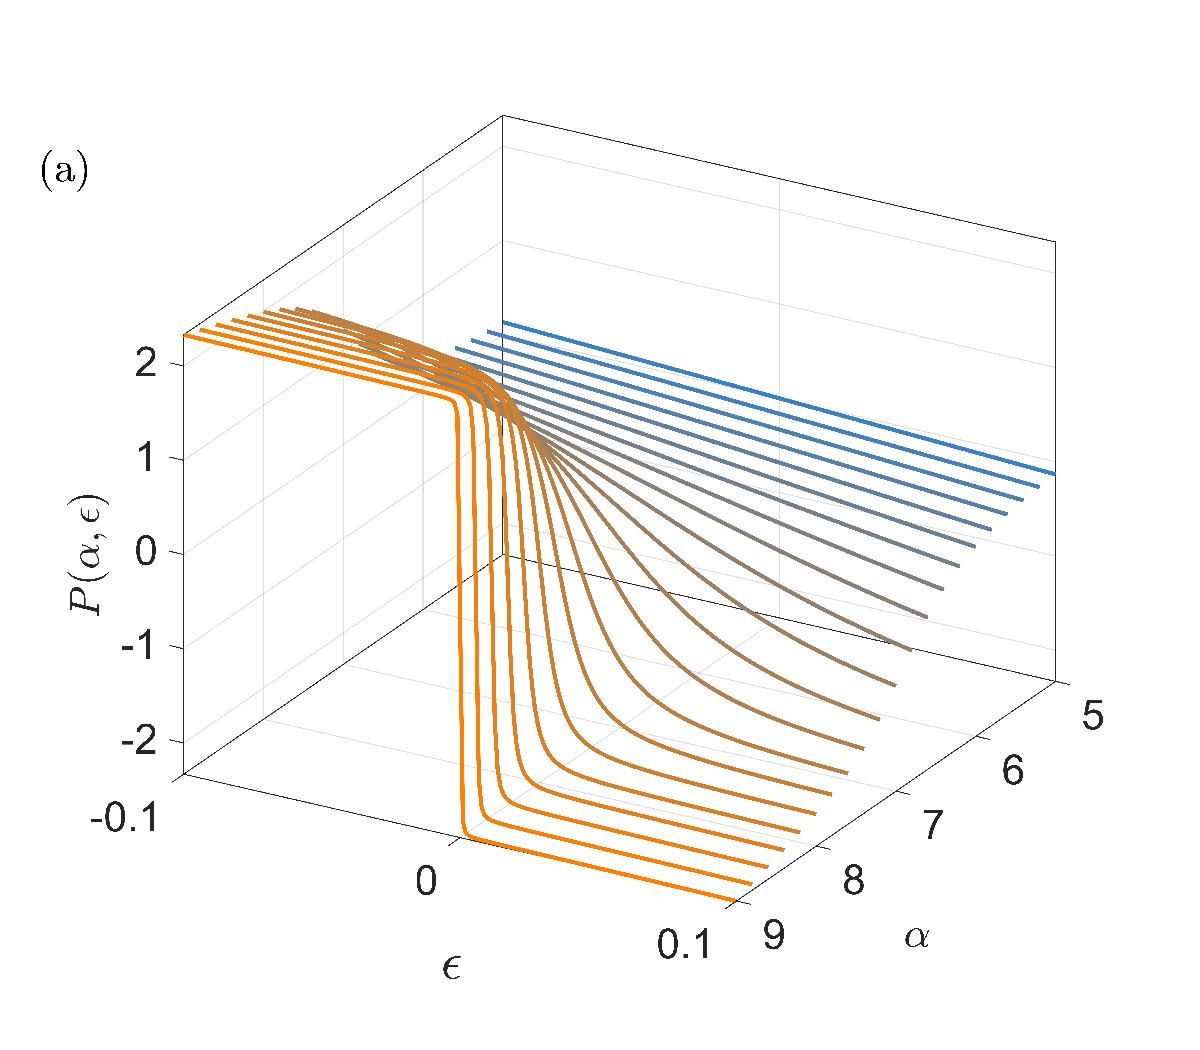
\includegraphics[width=1\columnwidth]{Fig_Polarization_3D_theor}
	\includegraphics[width=1\columnwidth]{Fig_Polarization_3D_exp}
     \caption{Top: Polarization as a function of $\alpha$ and $\epsilon$ as computed by exact diagonalization. Bottom:}
	\end{center}
\end{figure}


\subsection{Comparison with experiments}
\begin{itemize}
\item Scaling the experiments and the numerical data together
\end{itemize}

	
\section{Conclusion}
\begin{itemize}
\item Quantum fluctuations effects tunneling transition
\item transverse factor renormalize tunneling
\item Scaling with experimental data
\end{itemize}

  

     
 
\appendix
\section{•}
Some part of the ED and Instanton calculation would go here if it is too lengthy.

	
	
	


\bibliography{references}
\end{document}
